% Created 2017-04-28 五 22:53
\documentclass[11pt]{article}
\usepackage[utf8]{inputenc}
\usepackage[T1]{fontenc}
\usepackage{fixltx2e}
\usepackage{graphicx}
\usepackage{longtable}
\usepackage{float}
\usepackage{wrapfig}
\usepackage{rotating}
\usepackage[normalem]{ulem}
\usepackage{amsmath}
\usepackage{textcomp}
\usepackage{marvosym}
\usepackage{wasysym}
\usepackage{amssymb}
\usepackage{hyperref}
\tolerance=1000
\author{Qiu Wei}
\date{\today}
\title{MPML REPORT}
\hypersetup{
  pdfkeywords={},
  pdfsubject={},
  pdfcreator={Emacs 24.5.1 (Org mode 8.2.10)}}
\begin{document}

\maketitle
\tableofcontents

\begin{abstract}
to be finished
\end{abstract}


\section{Min-max algorithm}
\label{sec-1}
The min-max algorithm seperates the positive set and negative set into
small parts. For example, the positive set is partitioned to n parts and
the negative set to m parts, then build n*m svm models between these parts.
\ldots{}
\section{Parallelization}
\label{sec-2}

\section{Implementation}
\label{sec-3}
The python version is implemented with MPI,the source code is partitioned into several
parts via its functions. I will introduce the main structure of this project in the following.

\subsection{usage}
\label{sec-3-1}
To test a classifier, configure the algorithm in \emph{settings.py}. If min-max net algorithm
is used, specify the partition function in \emph{settings.py}, then run this command:
\begin{verbatim}
$ cd src/
$ python3 main.py
\end{verbatim}
In addition,if you want to run with the origin data, set PARSE\_DATA = True so
that the program will parse the origin data into .pickle files. The time of
parsing do not count in total time in timer class as you only need to parse the
data for just one time. Other advanced options can be found in the folloing part.

When all the algorithm have been tested, you can draw the ROC graph by \emph{drawroc.py}.
Run this command to draw ROC graph and calc AUC value:
\begin{verbatim}
$ python3 drawroc.py
\end{verbatim}

\subsection{structure}
\label{sec-3-2}
All the source code can be found in src/ folder. src/core/ stores the main part of
brute liblinear, serialized min-max and paralleled min-max algorithm. src/data/ stores
the training data, testing data and all the template .pickle files. src/models/ stores
all the svm models. src/tools/ stores many tool function for this project. src/timer/
contains timer class. src/utils/ contains util functions. src/settings.py contains
default settings. src/main.py is the main program. src/drawroc.py draw ROC graphs
via the result file in src/data/ folder.

\subsection{settings.py}
\label{sec-3-3}
The \emph{settings.py} file contains default settings of this project, containing default
algorithm, partition function in min-max algorithm,some constant and some folder/file name.
As there are no time to implement a parser, you must edit \emph{settings.py} to configure
the algorithm.

To start with, set the value of ALGORITHM
to specify which kind of algorithm you want and then set the value of PARTITION\_ALGORITHM to choose
partition function(labeled of randomed).

If you want to use post models for debugging, set MEMORIZE = True.
If you want to test the program in a smaller data set, set TRAIN\_DATA to your desired item numbers
greater than 0.
If you want to patition the items into a different number of sets in random labeled min-max net algorithm,
change the value of MAX\_CLASS to the max number of sets.

Other settings are seldom used and you can learn about their function by reading the source codes.

\subsection{utils and tools}
\label{sec-3-4}
The utils module comes from a repo in github, it mainly contains functional programming style
util functions such as partition, mapValue and mapv. A cd class is also contained to
ensure safe dictory switch.

src/tools stores the tools specificly designed for this project. \emph{partition.py} contains
partition functions used to partition data into different sets in min-max algorithm. \emph{dataIO.py}
implements the IO instruction with files. \emph{parseData.py} parses the origin data into a hash-map
in python, and dump it to a .pickle file. The main program will use the .pickle file directly
so this module will not be called in main program. \emph{tools.py} defines getModel, predictResult
,compareResult and metaNameFunc which will be used in all the three algorithms.

\subsection{drawroc.py}
\label{sec-3-5}
\emph{drawroc.py} use matplotlib.pyplot module to draw the ROC graph.
First it reads the result file of different algorithms, then call pyplot
to draw the ROC graph. Also the AUC value of the result is also calculated
and printed to the screen.
\subsection{timer}
\label{sec-3-6}
\emph{timer.py} uses time module to implement a multi-record timer. Different record
are stored in a hash-map and distinguished by its name. The start and end method
can start/end the timing a specific record. Also an add method is provided to
add a value to a record.
\subsection{core}
\label{sec-3-7}
The core module contains the main part of the program.
\emph{brute.py} use liblinear directly to solve the origin problem.
\emph{minmax.py} defines the abstraction of min-max algorithm and implements
the serialized version of this algorithm.
\emph{multiProc.py} implements the parallelized version of min-max algorithm.

\section{Trainning Result}
\label{sec-4}
The trainning result is as following:
\begin{center}
\begin{tabular}{rllrlrr}
\hline
No. & Algorithm & paralleled? & Time/s & Accuracy & F1 value & AUC value\\
\hline
1 & brute svm & $\backslash$ & 34.04 & 96.37167\% & 0.92404 & 0.48782\\
2 & random min-max & no & 305.47 & 96.26846\% & 0.92194 & $\backslash$\\
3 & random min-max & yes & 140.08 & 96.26846\% & 0.92184 & 0.48307\\
4 & labeled min-max & no & 204.35 & 96.71042\% & 0.93101 & $\backslash$\\
5 & labeled min-max & yes & 204.35 & 96.69719\% & 0.93074 & 0.48567\\
\hline
\end{tabular}
\end{center}
The random min-max algorithm separate the input data into 5 parts randomly(5*5 models).
The labeled min-max seperate the input data via the first two letters(4*12 models).

The total contains the time of load data, save model and other IO operations.
Parsing is finished before the program runs.

The ROC Graph is as following:


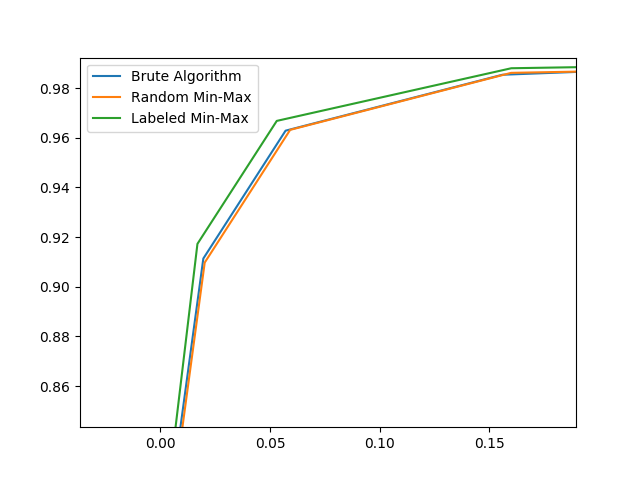
\includegraphics[width=.9\linewidth]{figure_1.png}



The time cost between serialized min-max and parallelized min-max is:

\begin{center}
\begin{tabular}{rlllll}
\hline
No. & Parallelized? & Algorithm & Trainning time & Testing time & Total time\\
\hline
1 & Yes & labeled & 59.37346 s & 144.54046 s & 203.93383 s\\
2 & No & labeled & 115.96271 s & 371.83840 s & 489.00508 s\\
3 & Yes & random & 54.49303 s & 84.16756 s & 138.69087 s\\
4 & No & random & 103.98813 s & 200.19163 s & 305.47026 s\\
\hline
\end{tabular}
\end{center}


Test environment is Ubuntu, 4 kernal.
Python version is 3.5.
\section{Analysis}
\label{sec-5}
% Emacs 24.5.1 (Org mode 8.2.10)
\end{document}